\documentclass{standalone}
\usepackage{tikz}
\usetikzlibrary{patterns, positioning}
\usepackage[sfdefault]{ClearSans} %% option 'sfdefault' activates Clear Sans as the default text font
\usepackage[T1]{fontenc}

\begin{document}
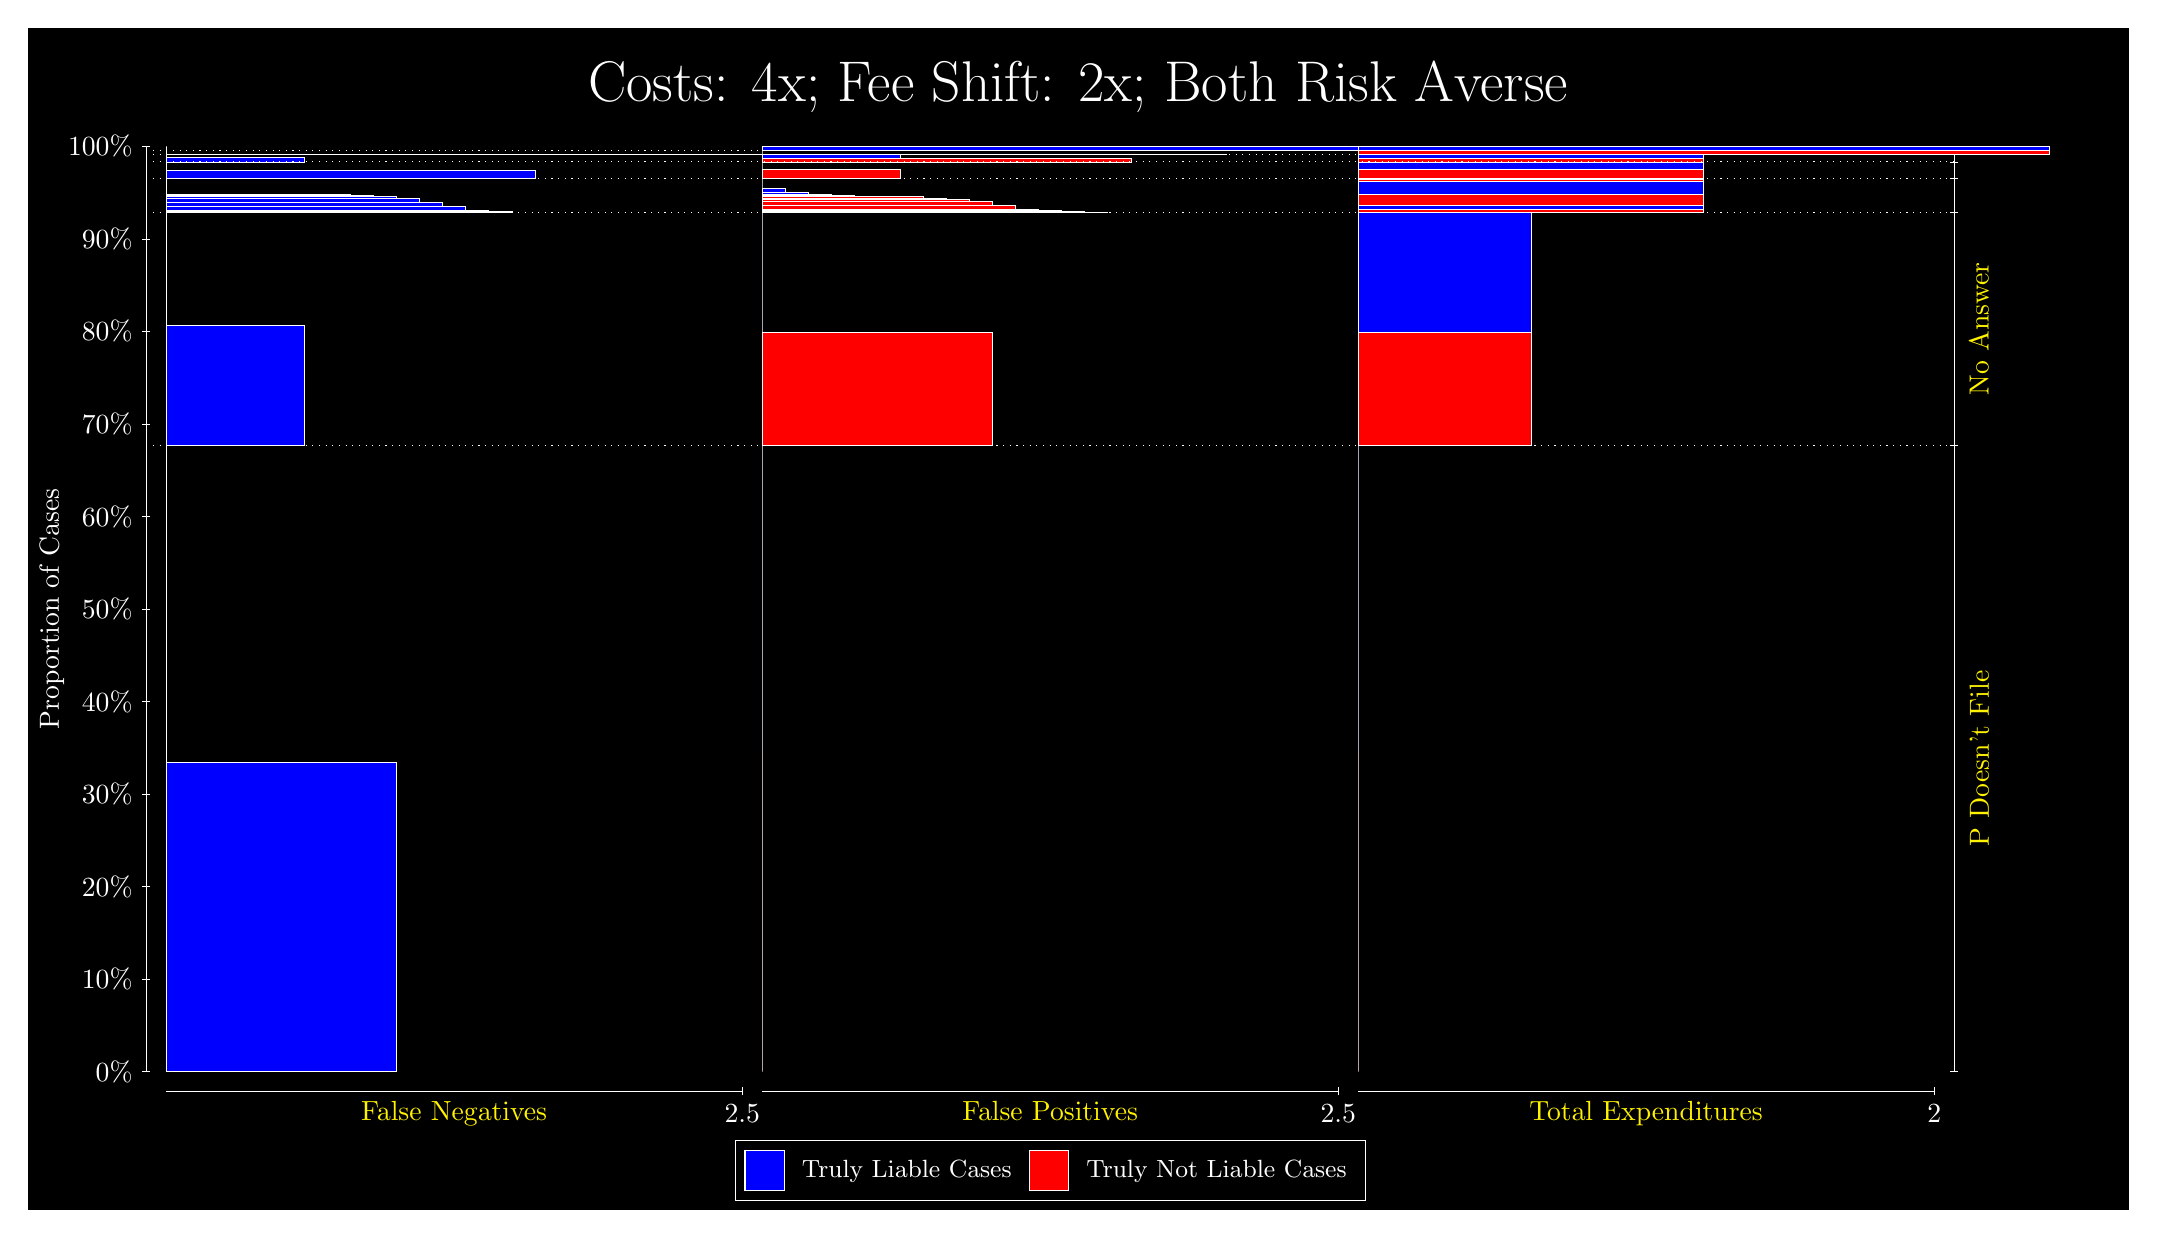
\begin{tikzpicture}
\draw[fill=black] (0,0) rectangle (26.667,15);
\draw[text=white] (0,13.5) rectangle (26.667,15) node[midway] {\huge Costs: 4x; Fee Shift: 2x; Both Risk Averse};
\draw[white, very thin] (1.5,1.75) -- (1.5,13.5);
\node[rotate=90, text=white, anchor=center] at (0.3, 7.625) {Proportion of Cases};
\draw[white, very thin] (1.45,1.75) -- (1.55,1.75);
\node[text=white, anchor=east] at (1.45, 1.75) {0\%};
\draw[white, very thin] (1.45,2.925) -- (1.55,2.925);
\node[text=white, anchor=east] at (1.45, 2.925) {10\%};
\draw[white, very thin] (1.45,4.1) -- (1.55,4.1);
\node[text=white, anchor=east] at (1.45, 4.1) {20\%};
\draw[white, very thin] (1.45,5.275) -- (1.55,5.275);
\node[text=white, anchor=east] at (1.45, 5.275) {30\%};
\draw[white, very thin] (1.45,6.45) -- (1.55,6.45);
\node[text=white, anchor=east] at (1.45, 6.45) {40\%};
\draw[white, very thin] (1.45,7.625) -- (1.55,7.625);
\node[text=white, anchor=east] at (1.45, 7.625) {50\%};
\draw[white, very thin] (1.45,8.8) -- (1.55,8.8);
\node[text=white, anchor=east] at (1.45, 8.8) {60\%};
\draw[white, very thin] (1.45,9.975) -- (1.55,9.975);
\node[text=white, anchor=east] at (1.45, 9.975) {70\%};
\draw[white, very thin] (1.45,11.15) -- (1.55,11.15);
\node[text=white, anchor=east] at (1.45, 11.15) {80\%};
\draw[white, very thin] (1.45,12.325) -- (1.55,12.325);
\node[text=white, anchor=east] at (1.45, 12.325) {90\%};
\draw[white, very thin] (1.45,13.5) -- (1.55,13.5);
\node[text=white, anchor=east] at (1.45, 13.5) {100\%};

\draw[white, very thin] (24.457,1.75) -- (24.457,13.5);
\draw[white, very thin] (24.407,1.75) -- (24.507,1.75);
\node[anchor=west] at (24.407, 1.75) {};
\draw[white, very thin] (24.407,9.7056) -- (24.507,9.7056);
\node[anchor=west] at (24.407, 9.7056) {};
\draw[white, very thin] (24.407,12.658) -- (24.507,12.658);
\node[anchor=west] at (24.407, 12.658) {};
\draw[white, very thin] (24.407,13.097) -- (24.507,13.097);
\node[anchor=west] at (24.407, 13.097) {};
\draw[white, very thin] (24.407,13.303) -- (24.507,13.303);
\node[anchor=west] at (24.407, 13.303) {};
\draw[white, very thin] (24.407,13.396) -- (24.507,13.396);
\node[anchor=west] at (24.407, 13.396) {};
\draw[white, very thin] (24.407,13.451) -- (24.507,13.451);
\node[anchor=west] at (24.407, 13.451) {};
\draw[white, very thin] (24.407,13.5) -- (24.507,13.5);
\node[anchor=west] at (24.407, 13.5) {};

\draw[white, very thin, fill=blue] (1.75,1.75) rectangle (4.6775,5.6736);
\draw[white, very thin, fill=red] (1.75,5.6736) rectangle (1.75,9.7056);
\draw[white, very thin, fill=blue] (1.75,9.7056) rectangle (3.5065,11.223);
\draw[white, very thin, fill=red] (1.75,11.223) rectangle (1.75,12.658);
\draw[white, very thin, fill=blue] (1.75,12.658) rectangle (6.1413,12.676);
\draw[white, very thin, fill=blue] (1.75,12.676) rectangle (5.8486,12.687);
\draw[white, very thin, fill=blue] (1.75,12.687) rectangle (5.5558,12.736);
\draw[white, very thin, fill=blue] (1.75,12.736) rectangle (5.2631,12.793);
\draw[white, very thin, fill=blue] (1.75,12.793) rectangle (4.9703,12.842);
\draw[white, very thin, fill=blue] (1.75,12.842) rectangle (4.6775,12.865);
\draw[white, very thin, fill=blue] (1.75,12.865) rectangle (4.3848,12.88);
\draw[white, very thin, fill=blue] (1.75,12.88) rectangle (4.092,12.886);
\draw[white, very thin, fill=blue] (1.75,12.886) rectangle (3.7993,12.891);
\draw[white, very thin, fill=red] (1.75,12.891) rectangle (1.75,13.097);
\draw[white, very thin, fill=blue] (1.75,13.097) rectangle (6.4341,13.195);
\draw[white, very thin, fill=red] (1.75,13.195) rectangle (1.75,13.303);
\draw[white, very thin, fill=blue] (1.75,13.303) rectangle (3.5065,13.355);
\draw[white, very thin, fill=red] (1.75,13.355) rectangle (1.75,13.396);
\draw[white, very thin, fill=blue] (1.75,13.396) rectangle (15.217,13.399);
\draw[white, very thin, fill=red] (1.75,13.399) rectangle (1.75,13.451);
\draw[white, very thin, fill=red] (1.75,13.451) rectangle (1.75,13.454);
\draw[white, very thin, fill=blue] (1.75,13.454) rectangle (1.75,13.5);
\draw[white, very thin, fill=red] (9.3189,1.75) rectangle (9.3189,5.782);
\draw[white, very thin, fill=blue] (9.3189,5.782) rectangle (9.3189,9.7056);
\draw[white, very thin, fill=red] (9.3189,9.7056) rectangle (12.246,11.14);
\draw[white, very thin, fill=blue] (9.3189,11.14) rectangle (9.3189,12.658);
\draw[white, very thin, fill=red] (9.3189,12.658) rectangle (13.71,12.663);
\draw[white, very thin, fill=red] (9.3189,12.663) rectangle (13.417,12.669);
\draw[white, very thin, fill=red] (9.3189,12.669) rectangle (13.125,12.684);
\draw[white, very thin, fill=red] (9.3189,12.684) rectangle (12.832,12.706);
\draw[white, very thin, fill=red] (9.3189,12.706) rectangle (12.539,12.752);
\draw[white, very thin, fill=red] (9.3189,12.752) rectangle (12.246,12.796);
\draw[white, very thin, fill=red] (9.3189,12.796) rectangle (11.954,12.833);
\draw[white, very thin, fill=red] (9.3189,12.833) rectangle (11.661,12.841);
\draw[white, very thin, fill=red] (9.3189,12.841) rectangle (11.368,12.863);
\draw[white, very thin, fill=blue] (9.3189,12.863) rectangle (10.783,12.869);
\draw[white, very thin, fill=blue] (9.3189,12.869) rectangle (10.49,12.875);
\draw[white, very thin, fill=blue] (9.3189,12.875) rectangle (10.197,12.89);
\draw[white, very thin, fill=blue] (9.3189,12.89) rectangle (9.9044,12.913);
\draw[white, very thin, fill=blue] (9.3189,12.913) rectangle (9.6116,12.962);
\draw[white, very thin, fill=blue] (9.3189,12.962) rectangle (9.3189,13.097);
\draw[white, very thin, fill=red] (9.3189,13.097) rectangle (11.075,13.204);
\draw[white, very thin, fill=blue] (9.3189,13.204) rectangle (9.3189,13.303);
\draw[white, very thin, fill=red] (9.3189,13.303) rectangle (14.003,13.343);
\draw[white, very thin, fill=blue] (9.3189,13.343) rectangle (11.075,13.396);
\draw[white, very thin, fill=red] (9.3189,13.396) rectangle (9.3189,13.447);
\draw[white, very thin, fill=blue] (9.3189,13.447) rectangle (9.3189,13.451);
\draw[white, very thin, fill=red] (9.3189,13.451) rectangle (22.786,13.454);
\draw[white, very thin, fill=blue] (9.3189,13.454) rectangle (19.858,13.5);
\draw[white, very thin, fill=red] (16.888,1.75) rectangle (16.888,5.782);
\draw[white, very thin, fill=blue] (16.888,5.782) rectangle (16.888,9.7056);
\draw[white, very thin, fill=red] (16.888,9.7056) rectangle (19.083,11.14);
\draw[white, very thin, fill=blue] (16.888,11.14) rectangle (19.083,12.658);
\draw[white, very thin, fill=red] (16.888,12.658) rectangle (21.279,12.703);
\draw[white, very thin, fill=blue] (16.888,12.703) rectangle (21.279,12.753);
\draw[white, very thin, fill=red] (16.888,12.753) rectangle (21.279,12.892);
\draw[white, very thin, fill=blue] (16.888,12.892) rectangle (21.279,13.056);
\draw[white, very thin, fill=red] (16.888,13.056) rectangle (21.279,13.076);
\draw[white, very thin, fill=blue] (16.888,13.076) rectangle (21.279,13.097);
\draw[white, very thin, fill=red] (16.888,13.097) rectangle (21.279,13.204);
\draw[white, very thin, fill=blue] (16.888,13.204) rectangle (21.279,13.303);
\draw[white, very thin, fill=red] (16.888,13.303) rectangle (21.279,13.343);
\draw[white, very thin, fill=blue] (16.888,13.343) rectangle (21.279,13.396);
\draw[white, very thin, fill=red] (16.888,13.396) rectangle (25.67,13.447);
\draw[white, very thin, fill=blue] (16.888,13.447) rectangle (25.67,13.451);
\draw[white, very thin, fill=red] (16.888,13.451) rectangle (25.67,13.454);
\draw[white, very thin, fill=blue] (16.888,13.454) rectangle (25.67,13.5);
\draw[white, dotted] (1.5,9.7056) -- (24.457,9.7056);
\draw[white, dotted] (1.5,12.658) -- (24.457,12.658);
\draw[white, dotted] (1.5,13.097) -- (24.457,13.097);
\draw[white, dotted] (1.5,13.303) -- (24.457,13.303);
\draw[white, dotted] (1.5,13.396) -- (24.457,13.396);
\draw[white, dotted] (1.5,13.451) -- (24.457,13.451);
\draw[white, very thin] (1.75,1.5) -- (9.0689,1.5);
\node[text=yellow, anchor=north] at (5.4094, 1.5) {False Negatives};
\draw[white, very thin] (9.0689,1.45) -- (9.0689,1.55);
\node[text=white, anchor=north] at (9.0689, 1.45) {2.5};

\draw[white, very thin] (9.3189,1.5) -- (16.638,1.5);
\node[text=yellow, anchor=north] at (12.978, 1.5) {False Positives};
\draw[white, very thin] (16.638,1.45) -- (16.638,1.55);
\node[text=white, anchor=north] at (16.638, 1.45) {2.5};

\draw[white, very thin] (16.888,1.5) -- (24.207,1.5);
\node[text=yellow, anchor=north] at (20.547, 1.5) {Total Expenditures};
\draw[white, very thin] (24.207,1.45) -- (24.207,1.55);
\node[text=white, anchor=north] at (24.207, 1.45) {2};

\node[text=yellow, centered, rotate=90] at (24.777, 5.7278) {P Doesn't File};
\node[text=yellow, centered, rotate=90] at (24.777, 11.182) {No Answer};






\draw (12.978300999999998,1.5) node[draw=none] (baseCoordinate) {};
\begin{scope}[align=center]
        \matrix[scale=0.5, draw=white, below=0.5cm of baseCoordinate, nodes={draw}, column sep=0.1cm]{
            \node[rectangle, draw, minimum width=0.5cm, minimum height=0.5cm, fill=blue] {}; &
            \node[draw=none, font=\small, text=white] (B) {Truly Liable Cases}; &
            \node[rectangle, draw, minimum width=0.5cm, minimum height=0.5cm, fill=red] {}; &
            \node[draw=none, font=\small, text=white] (B) {Truly Not Liable Cases}; \\
            };
\end{scope}

\end{tikzpicture}
\end{document}